% Anonymous ACLing 2026 submission draft.
% Prepared from the full Context-Aware Linguistic Steganography preprint.
\documentclass[3p,times,procedia]{elsarticle}
\flushbottom
\usepackage{ecrc}
\usepackage[bookmarks=false]{hyperref}
\hypersetup{colorlinks,linkcolor=blue,citecolor=blue,urlcolor=blue}
\usepackage{amsmath,amssymb}
\usepackage{booktabs}
\usepackage{array}
\usepackage{graphicx}
\usepackage{placeins}
\usepackage{flafter}
\usepackage{url}
\hyphenation{OPPRESSION}
\graphicspath{{figures/}}

\volume{00}
\firstpage{1}
\journalname{Procedia Computer Science}
\runauth{Anonymous}
\jid{procs}
\dochead{8th International Conference on AI in Computational Linguistics}

\begin{document}
\begin{frontmatter}

\title{Context-Aware Linguistic Steganography through Reply and Topic Selection}

\author{Anonymous Authors}
\address{Anonymous submission}

\begin{abstract}
Linguistic steganography usually embeds bits by changing token-generation probabilities. This paper studies a black-box alternative for threaded discussions: message bits select a reply target and a comment topic, and a language model writes an ordinary reply for those choices. Sender and receiver construct ordered lists from the post, its comments, and agreed domain texts. A sender-side verification loop rejects a reply when the receiver-style topic classifier does not recover the intended choice. We evaluate contextual quality, generation, and complete-message extraction under explicitly separated receiver conditions. On a selected 244-post judge set, our comments were chosen as the weakest text in 29.1\% of three-way tasks versus 47.5\% for the ZLG baseline and received higher register-fit scores (3.193 versus 2.791). ZLG was harder to identify in a ten-comment lineup (28.3\% versus 51.6\% detection). Complete-message recovery was 7/25 with prepared shared context and 5/6 on the anchored seven-attempt archive-development panel. These results support a contextual selection channel, while leaving live-platform delivery, adaptive steganalysis, and fully independent web/model reconstruction for future work.
\end{abstract}

\begin{keyword}
linguistic steganography \sep large language models \sep black-box generation \sep conversational context \sep message recovery
\end{keyword}
\end{frontmatter}

\section{Introduction}

Text steganography must hide both the message and the fact that communication is taking place. Text is difficult because it has little redundancy: a statistically unusual choice or a semantically misplaced sentence can expose the channel. Generative language models improve surface fluency, but a grammatical reply can still be conspicuous when it does not fit the post or the comment to which it responds \citep{ding2023context,liao2024co,wang2023hi}. Token-level methods address this problem by steering next-token sampling, but they normally require model probabilities or a shared tokenizer \citep{zhang2021provably,kaptchuk2021meteor}.

We study a black-box selection channel for threaded discussions. The sender and receiver build the same ordered reply-location and comment-topic lists. Message bits select one location and one topic; a language model then writes a visible reply suited to the selected context. The receiver reads the location and identifies the topic from the generated text. The method uses ordinary API access and does not insert invisible characters.

Our contributions are threefold. First, we define a two-layer selection channel that separates observable conversational choices from token probabilities. Second, we specify the shared context, ordering, synchronization, verification, and multi-comment transport needed to interpret those choices. Third, we evaluate comment quality, generation, and complete-message recovery while recording the receiver inputs available in each experiment. The work makes no theoretical security claim and does not treat sender-side audit reconstruction as independent public-text recovery.

\section{Related work}

Generative linguistic steganography usually hides a payload in token choices. Provably secure schemes and Meteor-style constructions need the model's next-token distribution or a shared tokenizer \citep{zhang2021provably,kaptchuk2021meteor}. Context-aware models ask whether a sentence belongs with the surrounding text, but they still typically encode bits inside generation \citep{ding2023context,liao2024co,wang2023hi}. Zero-shot generative linguistic steganography (ZLG) avoids task-specific training by coding bits in token probabilities during prompted generation. Its receiver needs a matching model, tokenizer, prompt, and codec \citep{lin2024zero}.

Black-box prompting is a separate design. LLM-Stega selects among prompted keywords and rejects a candidate when extraction feedback does not recover the intended keyword \citep{wu2024generative}. That rejection loop is a precedent for checking a candidate before accepting it. OPPRESSION takes a different route: the parties agree on public documents and a deterministic codebook, then a short pointer stands in for a long fragment of text that already exists \citep{zillien2024oppression}. OPPRESSION does not write a social-media comment or choose where that comment sits in a thread.

The channel in this paper is the pair of public choices: which comment is answered, and which topic the reply discusses. A dictionary built from shared documents can shorten a text payload, following the reference idea in OPPRESSION, but the carrier is the generated reply. Table~\ref{tab:mechanisms} separates these mechanisms. It does not rank their security.

\begin{table}[t]
\centering
\caption{Information-carrying choice and the coordination the receiver needs.}
\label{tab:mechanisms}
\begin{tabular}{lp{0.33\columnwidth}p{0.36\columnwidth}}
\toprule
Method & What carries the bits & Receiver coordination \\
\midrule
LLM-Stega & Prompted keywords, checked by extraction feedback & Shared keyword mapping and extraction prompt \\
ZLG & Token probabilities during prompted generation & Matching model, tokenizer, prompt, and codec \\
OPPRESSION & Pointer into existing public text & Agreed documents; another channel carries the pointer \\
This work & Reply location and comment topic & Ordered lists, cutoff, helper settings, and framing \\
\bottomrule
\end{tabular}
\end{table}

\section{Method}

\subsection{Communication model}

Alice selects a public post and prepares a bounded copy of its comments. Both parties collect the post, its comments, and agreed domain documents through a deterministic helper configuration. Topic extraction produces an ordered list
\[
\mathcal{A}=(a_0,\ldots,a_{A-1}),
\]
where each record contains a source quote, a topic description, a category, and a source reference. Reply locations form a depth-first ordered list of size $C$, including the post itself. The parties must agree on the source texts, their order, the helper model and prompt, the comment cutoff, and the list-construction rules. Hashes can expose input differences but cannot make changing web content identical.

\subsection{Comment cutoff}

Research, topic extraction, and writing take time, and new comments can arrive before the reply is published. If the receiver later reads every comment on the post, the reply-location list can contain comments the sender never saw, and the topic list can change with them. The parties therefore agree on an interval $T_{\mathrm{sync}}$ between the sender's copy of the comments and publication of the carrier. When the carrier appears at time $t_{\mathrm{publish}}$, the receiver keeps comments available at
\[
t_{\mathrm{publish}}-T_{\mathrm{sync}}
\]
and excludes the carrier and its descendants. The interval must cover research, writing, and verification. If the work finishes early, the sender waits. If it overruns the interval, the old copy is no longer the copy the receiver will rebuild. Publication times must be readable, and the parties need a rule for a comment timestamped exactly on the cutoff. The cutoff still cannot restore a comment that was edited or deleted after the sender's copy. A preserved version is required when those edits would change either list.

\subsection{Two-layer selection channel}

The first bit field selects the reply location and the second selects a topic. With fixed-width power-of-two subsets, the distinguishable selection budget per carrier is
\[
b=\lfloor\log_2 C\rfloor+\lfloor\log_2 A\rfloor.
\]
For example, three reply locations and five topics provide $1+2=3$ distinguishable bits. This is an available selection budget, not Shannon capacity and not a measurement of useful payload independently recovered by a receiver. Modulo reduction can map different bit patterns to the same choice, so the multi-comment writer restricts choices to invertible subsets.

The writer receives the post, the selected parent chain, the selected topic description and source excerpt, and a research excerpt. It generates candidate replies at nonzero temperature. Before publication, Alice applies the same topic-identification procedure used by the receiver and retains a candidate only when it identifies the selected topic and passes a contextuality check. This verifies a candidate under the sender's available conditions; it does not by itself establish public-text receiver recovery.

\subsection{Receiver procedure}

The reply location is visible. The receiver finds the parent in the same depth-first order and reads that index as the first bit field. The topic index is not printed in the reply. The implemented decoder embeds the comment with a shared sentence encoder, retrieves a preliminary set of nearby topics, reranks them by combining semantic similarity with lexical overlap, and asks the identification model for a line of the form \texttt{idx: N}. Identification uses its own sampling setting, separate from the nonzero temperature used for writing. The default prompt shows a bounded shortlist, not the entire topic list.

Sender acceptance requires that this procedure return the selected index with no fallback. The decoder used at extraction time may map a shortlist rank back to a canonical index, and it may use the nearest semantic candidate when no index can be parsed. Those fallbacks are not available to the sender's acceptance check. A matching hash can show that two lists differ. It does not supply the list the receiver failed to rebuild.

\subsection{Payloads and multiple comments}

A text payload may be protected and then compressed against a dictionary built from the post, the comment copy, and the domain documents. The dictionary is a separate object from the comment-topic list, even when both are built from the same texts. One representation uses either raw UTF-8 or literals and pointers into that dictionary, and keeps the dictionary form only when it is shorter. Keyed modes can hide the payload bytes. They do not hide the fact that a comment was published.

A single comment carries only the choices available in its two lists. A longer comment does not add bits to those fields. Larger messages therefore use several carriers. Let $P$ be the prepared payload, $L$ its length in bits, and $N$ the number of carriers. The implemented stream is
\[
S=M\Vert V\Vert\Gamma(N)\Vert\Gamma(L)\Vert P\Vert R,
\]
where $M$ is a 16-bit recognition marker, $V$ is a 2-bit version, $\Gamma$ is Elias gamma coding, and $R$ is a CRC-32 check of $P$. The marker and version occur once per message, not once per comment, and they may cross a comment boundary. The planner accepts the smallest $N$, within a configured limit, whose invertible selection budgets cover $S$ including the gamma fields. The final carrier may be padded with zeros; the length and check tell the receiver where the padding starts.

The receiver joins candidate bit slices in the supplied order. It rejects a missing carrier, an inconsistent count or length, a failed CRC, or nonzero bits where padding is required. Reading most carriers correctly is not a recovered message when the remaining choices break the check. The carrier limit bounds how many comments the parties will write and read. It does not define an optimal message size, and this implementation does not discover the bundle from the public thread by itself.

\begin{figure}[t]
\centering
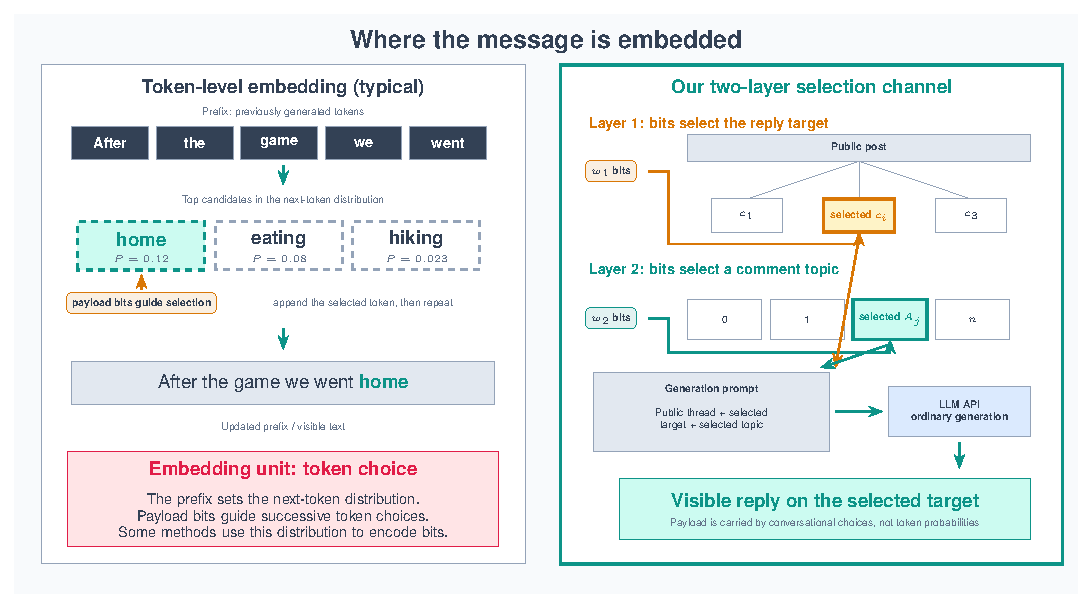
\includegraphics[width=\columnwidth]{token_vs_intent_embedding}
\caption{Token-level embedding compared with the proposed two-layer selection channel. Bits select a reply location and a conversational topic before the model writes the visible reply.}
\label{fig:selection-channel}
\end{figure}

\section{Experimental design}

The experiments answer different questions and are not one benchmark. The initial configuration comparison used 304 accepted pairs over 100 source posts and compared an available selection budget with a reported ZLG payload. The comment-quality study used one eligible pair for each of 244 posts selected from a frozen 1,608-pair collection; 95 posts without a unique ZLG output were excluded. Five blinded tasks reused these same post-level pairs.

Complete-message experiments use different receiver contracts. The source-excerpt study assigned 25 messages selected from prepared source texts, so the payloads favor dictionary matches. The independent-payload development check assigned eight-byte messages and stopped after its third failure. Archive reconstruction independently prepared thread-only lists from public archive inputs. These experiments test different dependencies and are reported separately.

The quality judge was a single language model with five task-specific prompts. The tasks measured standout detection, weakest-text selection, suspicion AUROC, thread attribution, and register fit. Higher standout detection is worse for imperceptibility; the task is not a security test. Lineups were seeded, and the judge model is not deterministic. The scores are not a reader study. The baseline is official Zero-shot Generative Linguistic Steganography (ZLG), whose token-probability channel and receiver inputs differ from ours \citep{lin2024zero}.

The comment-quality comparison used local models from the Qwen 3.5 9B family for both methods, so a difference in model scale would not by itself explain the scores. Sharing a family does not make quantization, runtime, or retry policy identical, and the comparison did not replace our writer with a larger model. ZLG needs token probabilities. Our writer and topic identifier call a model through an API, so the design can use a service that does not expose those probabilities. The reported runs do not measure that broader choice.

Both quality comparisons rebuild our bitstrings from sender audit metadata. The decoder may take the recorded topic index instead of identifying it from the comment. The ZLG reveal in those runs received the sender's token identifiers and an externally supplied payload length. Each method therefore received different assistance. The comparisons do not decide which method a receiver can read from public text alone, and they use the single-comment path. ZLG can carry further bits by generating further tokens, within its acceptance limits. Our selection budget grows only when another comment supplies another location and topic. The initial comparison's capacity-matched setting rounded a per-sample budget to bytes and gave ZLG a payload excerpt. The 16.00 bits reported there are that setting, not ZLG's maximum.

Table~\ref{tab:contract} records the narrower contract of the source-excerpt experiment. The receiver sees the reply text and the comment and parent identifiers. It also receives a prepared copy of the comments, the ordered topic list, the dictionary, and the codec settings. Carrier order and sender identity are supplied. The original message, the intended indices, and the sender's acceptance traces are withheld until after decoding, when the recovered bytes are compared with the assigned text.

\begin{table}[t]
\centering
\caption{Receiver inputs in the source-excerpt extraction experiment.}
\label{tab:contract}
\begin{tabular}{lp{0.72\columnwidth}}
\toprule
Class & Supplied to the receiver \\
\midrule
Public & Reply text, with comment and parent identifiers \\
Shared setup & Prepared comment copy, ordered topic list, dictionary, and codec settings \\
Supplied order & Carrier references and sender identity; the length is read from the framing \\
Withheld & Original message, intended indices, and sender-acceptance traces \\
\bottomrule
\end{tabular}
\end{table}

\section{Results}

\subsection{Comment quality}

Table~\ref{tab:judge} summarizes the selected 244-post judge set. The results are criterion-specific. ZLG was harder to identify as the inserted comment, while our method was selected less often as the weakest text and scored higher on register fit. The AUROC values were close. The selected subset and one judge model limit the strength of these conclusions. On the parent freeze of 1,608 pairs over 339 posts, the mean available selection budget was 13.42 bits per comment and the mean reported ZLG payload was 13.90. Mean word counts were 23.86 and 15.91. Those bit figures are an available budget and a reported payload under audit assistance. They are not independently recovered useful payload.

\begin{table}[t]
\centering
\caption{Blinded LLM-judge results on 244 selected post pairs.}
\label{tab:judge}
\begin{tabular}{lcc}
\toprule
Criterion & Our method & ZLG \\
\midrule
Standout detection (lower is better) & 51.6\% & 28.3\% \\
Weakest text selected (lower is better) & 29.1\% & 47.5\% \\
Suspicion AUROC (lower is closer to human) & 0.661 & 0.650 \\
Thread attribution (higher is better) & 89.3\% & 75.0\% \\
Register fit, 1--5 (higher is better) & 3.193 & 2.791 \\
\bottomrule
\end{tabular}
\end{table}
\FloatBarrier

\subsection{Initial configuration comparison}

Table~\ref{tab:initial} is an earlier configuration experiment, not the 244-post judge set. Our method attempted 627 samples and accepted 554 (88.4\%). The failures were 70 topic mismatches and 3 generation failures. ZLG was then run on those 554 successes with a capacity-matched excerpt. The metric table uses the 304 accepted pairs, averaged over 100 source posts. The topic list was capped at 32, so the topic field contributed at most five bits to the selection budget. Our rows were reconstructed from sender audit metadata. ZLG has the lower GPT-2 perplexity and the higher reported bit figure. Our replies are longer and score higher on the run's lexical-quality index. BERTScore F1, measured against a human reference comment, is close. GPT-2 perplexity means predictability under GPT-2. It is not a human-quality score, and this table does not measure public-text recovery.

\begin{table}[t]
\centering
\caption{Initial configuration comparison over 100 source posts.}
\label{tab:initial}
\begin{tabular}{lcc}
\toprule
Metric & Our method & ZLG \\
\midrule
Selection budget / reported payload & 15.14 & 16.00 \\
GPT-2 perplexity (lower is more predictable) & 68.15 & 53.70 \\
Lexical quality index, 0--100 & 99.36 & 98.45 \\
Word count & 22.4 & 17.3 \\
BERTScore F1 & 0.842 & 0.848 \\
\bottomrule
\end{tabular}
\end{table}

\subsection{Generation and message recovery}

The source campaign permitted one retry and produced 2,543 accepted comments from 4,044 attempts. The 1,501 failures were 846 generation failures, 613 topic mismatches, and 42 invalid JSON responses. The balanced profile allows six retries after the first attempt, so this rate describes a lower-retry configuration. Every recorded success was reconstructed from sender audit metadata. That check shows the sender could regenerate its own bitstring. It does not show a receiver reading a public thread.

In the source-excerpt experiment, 7 of 25 assigned messages were recovered exactly with prepared shared context. Five attempts failed generation and 13 failed receiver recovery. Among the 20 complete generated sequences, recovery was 7/20. Across the 149 carriers in those sequences, 124 topic selections were correct and 25 were confused even though the intended topic remained in the shortlist. Every receiver-failed message included at least one such confusion, and in 23 confused frames the recorded prompts matched. Codebook and dictionary comparisons found no identity disagreement on the complete traces. All 25 offline codec and transport checks passed. The all-attempt proportion is 28\%, with a 95\% Wilson interval of 14.3\% to 47.6\% on this convenience batch. The interval does not estimate reliability for a broader population. Figure~\ref{fig:recovery-stages} keeps the message counts and the carrier counts separate: a high share of correct carriers can still leave the message unrecovered.

\begin{figure}[t]
\centering
\includegraphics[width=\columnwidth]{october_recovery_stages}
\caption{Source-excerpt recovery. The left panel counts all 25 assigned messages. The right panel counts topic selections only inside the 20 complete generated sequences.}
\label{fig:recovery-stages}
\end{figure}
\FloatBarrier

The independent-payload development check recovered 4 of 7 attempted messages before a prespecified no-go condition; three messages were left unattempted. All attempted messages generated, but incorrect topic classifications prevented complete recovery in three cases. This separates linguistic choice identification from transport correctness.

The archive panels independently rebuilt a deterministic thread-only list from a public archive. Each panel has six posts and an independent eight-byte message. The receiver derives the comment cutoff from the agreed timing window and does not receive the sender's codebook, expected hashes, payload length, or private carrier order. A separate driver performs that filtering. The production receiver does not yet discover carriers on a live platform. Table~\ref{tab:archive} compares three sender policies on the same posts. Two attempts recover 3/6 development messages and 2/6 untouched messages. Seven attempts recover 5/6 and 4/6. A concise rule, which keeps a reply only when it is no worse on a parent-similarity proxy and then prefers fewer words, preserves those exact counts and reduces all-attempt words by 4.07\% and 3.11\%. Pairwise writing judgments did not establish a quality improvement or preservation. Incomplete sequences ran out of generation attempts. They did not disagree on the public lists. These panels do not evaluate live Reddit publication, public discovery, complete web and model reconstruction, or adaptive attacks.

\begin{table}[t]
\centering
\caption{Archive reconstruction on six posts per panel. Word counts include attempts that did not recover the message.}
\label{tab:archive}
\begin{tabular}{llrr}
\toprule
Panel & Policy & Exact & Words \\
\midrule
Development & Two attempts & 3/6 & 1{,}935 \\
Development & Seven attempts & 5/6 & 2{,}752 \\
Development & Concise, seven attempts & 5/6 & 2{,}640 \\
Untouched & Two attempts & 2/6 & 1{,}277 \\
Untouched & Seven attempts & 4/6 & 2{,}186 \\
Untouched & Concise, seven attempts & 4/6 & 2{,}118 \\
\bottomrule
\end{tabular}
\end{table}

\section{Limitations and conclusion}

The evidence is configuration-specific. The judge uses a selected unique-output subset and one non-deterministic evaluator; its task outcomes are not independent samples. The initial comparison and comment-quality study use audit-assisted reconstruction, while the message experiments expose prepared or independently acquired inputs under separate contracts. The archive driver simulates public observation locally and does not implement full platform discovery. The paper therefore does not claim general steganographic security, resistance to editing, or complete end-to-end platform deployment.

The results show that conversational choices can serve as a black-box carrier when the parties can reconstruct compatible lists. They also show that receiver topic identification, rather than bit assembly alone, is a central failure point. Future work should test larger models, live platform delivery, independent search and model reconstruction, complete-message bundle detectability, and dedicated editing and steganalysis attacks.

\bibliographystyle{elsarticle-harv}
\bibliography{bibliography}

\end{document}

